\documentclass[a4paper,12pt]{article}
\usepackage[utf8]{inputenc}
\usepackage[spanish]{babel}
\usepackage{color}
\usepackage{parskip}
\usepackage{graphicx}
\usepackage{multirow}
\usepackage{listings}
\usepackage{vmargin}
\graphicspath{ {imagenes/} }
\definecolor{mygreen}{rgb}{0,0.6,0}
\definecolor{lbcolor}{rgb}{0.9,0.9,0.9}
\usepackage{epstopdf}



\begin{document}
\title{An Efficient Parallel Algorithm for Secured Data Communications Using RSA Public Key Criptography Method}
\author{
Christofer Fabián Chávez Carazas \\
\small{Universidad Nacional de San Agustín} \\
\small{Algoritmos Paralelos}
}

\maketitle

\section{Problema}

RSA es un algoritmo en encriptación y desencriptación con llave publica
basado en exponenciación y factorización de enteros con números muy largo,
de unos 1024 bits. El algoritmo secuencial de RSA consume mucho tiempo y energía.
Además, es difícil computar enteros muy grandes en la infraestructura GCC.

\section{Propuesta}

El paper propone un algoritmo paralelo para RSA implementado con la libreria
GMP y con la librería OpenMP en la infraestructura GCC.

\section{RSA}

RSA es uno de los algoritmos más importantes hoy en día en la encriptación
y la autenticación de datos transmitidos por toda la internet. RSA esta basado 
en la factorización de números muy largos, esto provee una fuerte seguridad.
RSA esta dividido en tres partes: Generación de las Keys, Encriptación y Desencriptación.\\

\section{Parallelization of RSA}

En el paper implementan un algoritmo paralelo para la exponenciación modular
usando dos tecnologías: GNU MP; para implementar las tres partes del RSA, y OpenMP para paralelizar el algoritmo
y obtener mayor rendimiento.

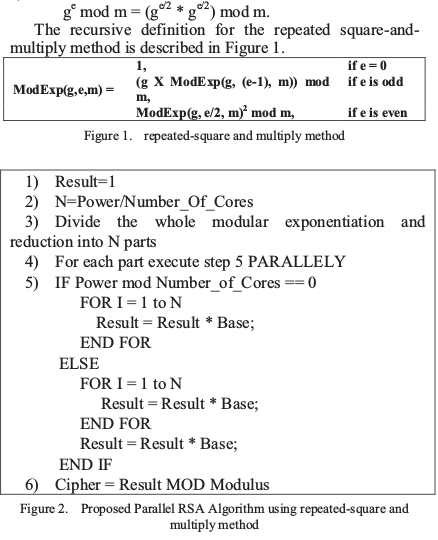
\includegraphics[scale = 0.5]{1.png}

\section{Experimentos}

\subsection{SetUp}
\begin{itemize}
 \item Procesador: AMD FX(tm)-8120 Eight-Core Processor 3.10 GHz
 \item RAM: 4,00 GB
 \item O.S.: Ubuntu Linux 11.04
 \item Platform: GCC Infraestructure
\end{itemize}

\subsection{Test Case Set 1}

Tamaño de keys: 128 a 1280
Tamaño de mensaje: 5000 caracteres.

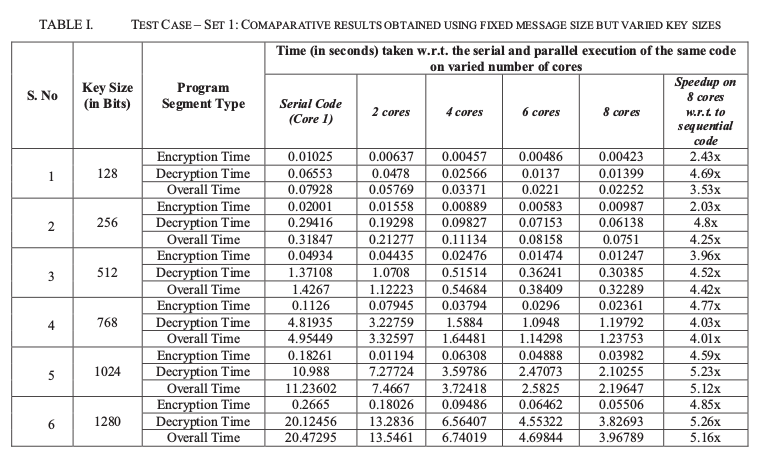
\includegraphics[scale = 0.5]{2.png}

\subsection{Test Case Set 2}

Tamaño de keys: 1024
Tamaño de mensaje: 1000 a 6000

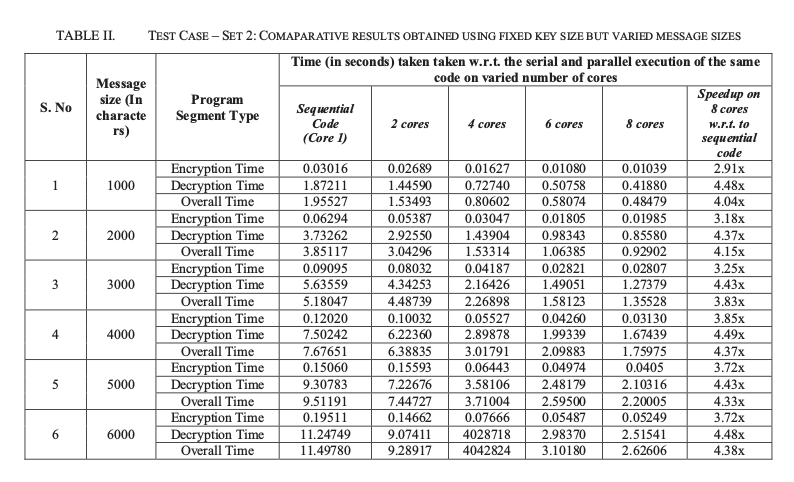
\includegraphics[scale = 0.5]{3.png}

\end{document}
